\section{Methodology}
%\KZ{Make figure \ref{fig:model} bigger, fonts bigger too. OK}
%Section \ref{sec:Methodology} describes our proposed MESDA framework in detail.
The proposed MICK framework contains a task enrichment method to
aggregate cross-domain knowledge, and a support classifier scheduled by
a fast-slow learner strategy to extract intra-support knowledge (illustrated in Figure \ref{fig:model}).
Next we present the structure and the learning process of MICK.
%We present the structure and the learning process of MESDA as follows.
%The framework is illustrated in Figure \ref{fig:model}.


\label{sec:Methodology}
\begin{figure*}[ht]
    \centering
    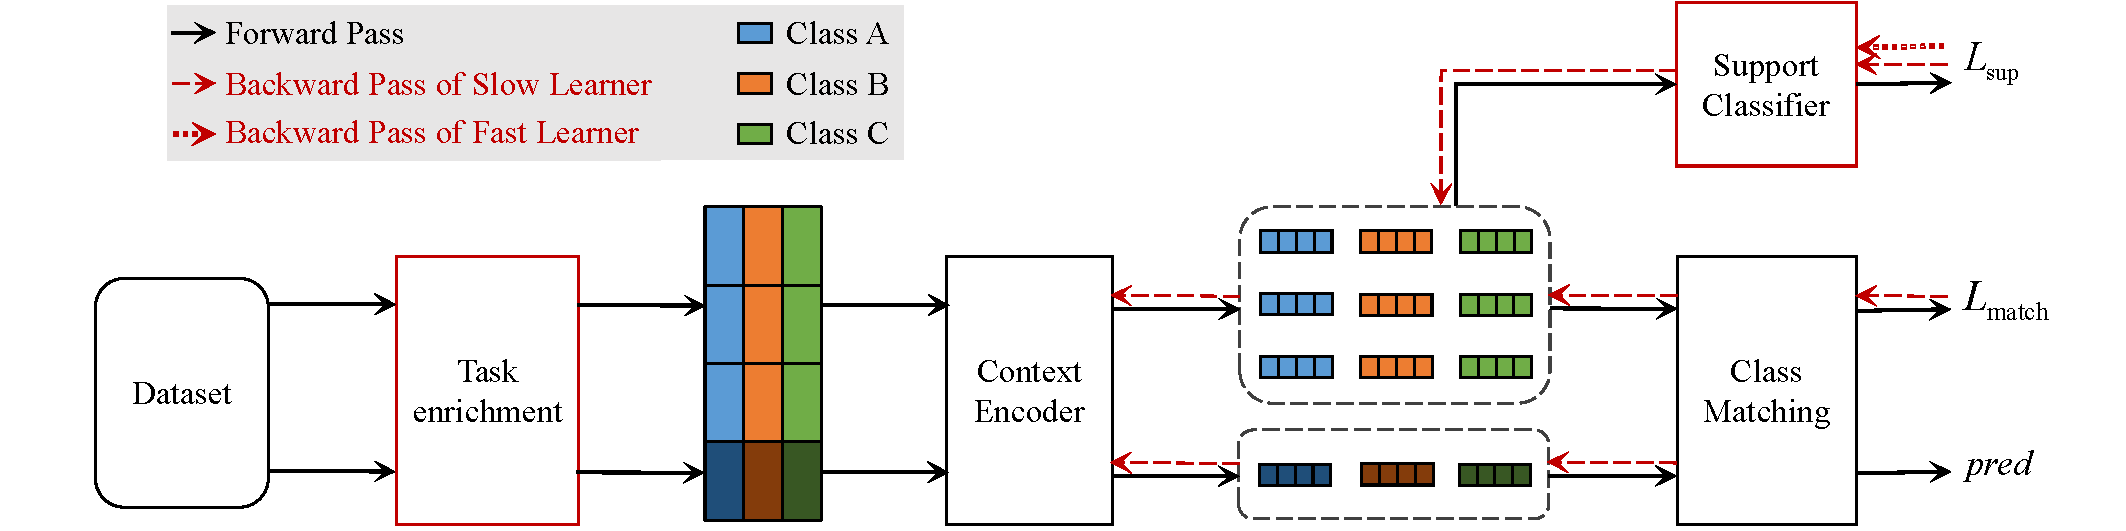
\includegraphics[width=17cm]{model.pdf}
    \caption{The structure and learning process of the MICK framework (under a 3-way 3-shot example). Modules with black border are typical meta-learning components. Modules with red border are our improvement. Cells of different colors represent instances from different classes. Light colors represent support instances. Dark colors represent query instances.
    %Solid lines, dash lines, and dotted lines represent forward pass, backward pass of slow learner, and backward pass of fast learner, respectively.
    }
    \label{fig:model}
\end{figure*}


\subsection{Overview of MICK}
\label{sec:structure}
As is shown in Figure \ref{fig:model},
%\KZ{Add the data augmentation into the fig as well}
the structure of our framework
consists of four main parts: {\em task enrichment}, {\em context encoder}, {\em class matching}
and {\em support classifier}.
%\KZ{Talk about the relations between these components and why you need them,
%especially why you need the supplimentary classifier, fast slow learner,
%and data augmentation.}
%As is shown in Figure \ref{fig:model}, the structure of our framework consists of three main parts: context encoder, class matching and supplementary classifier.
%\subsubsection{Context encoder}
%A support or query instance can be represented as a triple $(s, e, r)$, where $s$ is the sentence containing two entities $e=(e_1,e_2)$, and $r$ is the relation between $e_1$ and $e_2$. $r \in R$ where $R=\{r_1,...,r_N\}$ is the set of all candidate relation classes within one task and $N$ is the number of candidate classes.
%Sentence $s=\{c_0,..., c_i, ... c_{T-1}\}$ is of length $T$, where $c_i$ represent the one-hot vector of the $i^{th}$ character.
%In context encoder, each $c_i$ is mapped into a $d_c$ dimensional character embedding $\bm{x_i}$.
%To integrate positional information of $e_1$ and $e_2$ to each character, for each $c_i$, which is $d_1^i$ and $d_2^i$ characters away from $e_1$ and $e_2$ respectively, we map $d_1^i$ and $d_2^i$ to $d_p$ dimensional position embeddings $\mathbf{d}_1^i,\mathbf{d}_2^i$.
%$c_i$ is finally represented as the concatenation of the character embedding and the position embeddings, i.e., $\mathbf{u}_i=[\mathbf{x}_i,\mathbf{d}_1^i,\mathbf{d}_2^i]$.
%The representation matrix of sentence $s$ can be written as $\mathbf{U}=[\mathbf{u}_0,..., \mathbf{u}_i, ... ,\mathbf{u}_T]\ \mathrm{where}\ \mathbf{U} \in \mathbb{R}^{T\times (d_c + 2  d_p)}$, which is the concatenation of the representation vectors of the characters.

During training with task enrichment, for each episode, we randomly select a 
$N$-way $K$-shot task composed of $N \times K$ support instances and several query instances extracted from both the original training set $D_{\rm{train}}$ and supplementary cross-domain dataset.
Task enrichment enables the context encoder to learn cross-domain underlying knowledge.
The instances are first fed into the context encoder, which generates representation vectors for each instance.
Then we forward the encoded support and query vectors to class matching. Class matching aims to classify the query instances according to the representations of support instances.
Additionally, the support vectors are fed into a support classifier, which is a $N$-way linear classifier.
The support classifier aims to extract knowledge within support instances to facilitate the context encoder.
The back propagation process is scheduled by a fast-slow learner. Fast-slow learner scheme is motivated by meta-learner based meta learning methods \cite{Andry2016,Finn2017,HN} where the traditional learner and meta-learner learn with different speed. Task-specific parameters in the support classifier update every episode with a fast learner. Task-agnostic parameters in the context encoder update every $\epsilon$ episodes with a slow learner.
%The fast-learner aims to train the support classifier to quickly adapt to new classification tasks, while the slow learner helps the context encoder to fit all tasks.
With the fast-slow learner, we obtain a support classifier which can quickly adapt to new classification tasks and a global context encoder that fits all tasks.

During testing, we only use the context encoder and class matching method to make predictions on $D_{\rm{test}}$.

\subsection{Preliminaries}
%\KZ{Here you talk about the ordinary part of \figref{fig:model},
%i.e. how ordinary metalearning works.}
%A support or query instance can be represented as a triple $(s, e, r)$, where $s$ is the sentence containing two entities $e=(e_1,e_2)$, and $r$ is the relation between $e_1$ and $e_2$. $r \in R$ where $R=\{r_1,...,r_N\}$ is the set of all candidate relation classes within one task and $N$ is the number of candidate classes.
Modules in black boxes in Figure \ref{fig:model} compose an ordinary meta-learning framework.

For an instance $(s,e,r)$, sentence $s=\{c_0,..., c_i, ... c_{T-1}\}$ is padded to a predefined %of 
length $T$, where $c_i$ represents the one-hot vector of the $i^{th}$ word.
In context encoder, each $c_i$ is mapped to an embedding $\mathbf{x}_i \in \mathbb{R}^{d_c + 2 d_p}$, where $d_c$ is the word embedding\footnote{Character embedding for Chinese corpus.} size and $d_p$ is the position embedding size.
%each $c_i$ is mapped into a $d_c$ dimensional character embedding $\bm{x_i}$.
%To integrate positional information of $e_1$ and $e_2$ to each character, for each $c_i$, which is $d_1^i$ and $d_2^i$ characters away from $e_1$ and $e_2$ respectively, we map $d_1^i$ and $d_2^i$ to $d_p$ dimensional position embeddings $\mathbf{d}_1^i,\mathbf{d}_2^i$.
%$c_i$ is finally represented as the concatenation of the character embedding and the position embeddings, i.e., $\mathbf{u}_i=[\mathbf{x}_i,\mathbf{d}_1^i,\mathbf{d}_2^i]$.
The representation matrix of sentence $s$ is the concatenation of $\mathbf{x}_i$: $\mathbf{X}=[\mathbf{x}_0,..., \mathbf{x}_i, ... ,\mathbf{x}_{T-1}]$. $\mathbf{X} \in \mathbb{R}^{T\times (d_c + 2  d_p)}$.
%, which is the concatenation of the representation vectors of the characters. $\mathbf{X} \in \mathbb{R}^{T\times (d_c + 2  d_p)}$.

$\mathbf{X}$ is further fed into a sentence encoder (e.g., CNN or LSTM) to extract semantics of sentence $s$ and get representation vector $\mathbf{E} \in \mathbb{R}^{d_h}$, where $d_h$ is the dimension of hidden states.
%Conventional encoders include convolutional neural networks (CNNs) and long short-term memories (LSTMs). Encoders aggregated with attention have been proposed in recent years.
%During implementation, we follow \cite{ye-ling-2019-multi}, which facilitates the CNN encoder with local and instance-level attention.
%The output of the encoder
%(after pooling)
%is denoted as $\mathbf{E} \in \mathbb{R}^{d_h}$ where $d_h$ is the dimension of the hidden states.
Thus, an instance can be represented as a pair $(\mathbf{E},r)$, where $\mathbf{E}$ is the representation vector and $r$ is the relation class.


%For each relation $r_i \in R$, the support set $S$ contains a subset of $K$ instances of relation $r_i$, represented as $S^i=\{(\mathbf{E}^1,r_i),...,(\mathbf{E}^K, r_i)\}$. A centroid $\mathbf{C}^i$ is calculated with some aggregation function $\mathcal{A}$ over $S^i$, i.e., $\mathbf{C}^i=\mathcal{A}(\mathbf{E}^1, ..., \mathbf{E}^K)$ and $\mathbf{C}^i \in \mathbb{R}^{d_h}$.

Given an encoded query instance $Q=(\mathbf{E}^q, r^q)$ where $r^q$ is to be predicted, class matching aims to match $r^q$ with some relation class $r_i \in R$. Conventionally, a function $\mathcal{F}$ is adopted to measure the distance between $\mathbf{E}^q$ and $\mathbf{E}^{i}$, where $\mathbf{E}^{i}$ is the representation vector of relation $r_i$ and is calculated with all the representation vectors of support instances belonging to class $r_i$.
$\mathcal{F}$ can be a function either without parameters (e.g., Euclidean distance function) or with parameters (e.g., a linear classifier).
Relation class $r_i$ is chosen as the prediction class if $\mathbf{E}^i$ has the closest distance to $\mathbf{E}^q$.
%, i.e., $min(\{\mathcal{D}(\mathbf{E}^q, \mathbf{C}^{j})\}_{j=1}^N)=\mathcal{D}(\mathbf{E}^q, \mathbf{C}^{i})$.
%The relation $r_i$ with the closest distance $\mathcal{D}(\mathbf{E}^q, \mathbf{C}^{i})$ is chosen as the matched relation class.


%The function of class matching is to match an encoded query instance $(\mathbf{E}^q, r^q)$ to a certain class in $R$ given the encoded support set $S$. $S$ can be divided into $N$ subsets according to the relation class of instances: $S=\{S^{1},...,S^{N}\}$ where $S^{i}$ is the set of all instances in the support set with relation $r_i$. $S^{i}=\{(\mathbf{E}^{i}_1, r_i),...,(\mathbf{E}^{i}_K, r_i)\}$ where $r^i \in R$ and $K$ is the number of instances per relation class in the support set. In metric-learning based meta-learning methods, class matching is chiefly conducted by calculating the distance between support vectors and query vectors. Thus, no parameters are contained in this component.

%For the representation vectors $\{\mathbf{E}_1^i, ..., \mathbf{E}^i_K\}$ with the same relation $r_i$, a centroid $\mathbf{C}^i$ is calculated with some aggregation function $\mathcal{A}$, i.e $\mathbf{C}^i=\mathcal{A}(\mathbf{E}_1^i, ..., \mathbf{E}_K^i)$.
%For a query vector $\mathbf{E}^q$, a distance function $\mathcal{D}$ is adopted to calculate the distance between $\mathbf{E}^q$ and each centroid $\mathbf{C}^{i}$. The relation $r_i$ with the closest distance $\mathcal{D}(\mathbf{E}^q, \mathbf{C}^{i})$ is chosen as the prediction.

%A naive way of choosing $\mathcal{A}$ and $\mathcal{D}$ is to use mean function and Euclidean distance \cite{proto} respectively. During implementation, we follow \cite{ye-ling-2019-multi} to make $\mathcal{A}$ a weighted sum function and adopt their proposed class-level matching function.

\subsection{Task Enrichment}
\label{sec:data}
%\KZ{You haven't said what is supplementary data? Where do I obtain such data... This section needs to be passed again carefully.}
%Data augmentation expands the size of training data with supplementary data, which stands for open-source labeled data under the same task (here, the relation classification task). Common language is required between supplementary data and the training set despite the domain. Supplementary data can be obtained from other released datasets or online resources.
In order to expand the size of training data and enrich training tasks, we utilize cross-domain relation classification datasets in the same language. These datasets are obtained from released data of other works or online resources. This task enrichment step is necessary under the circumstance of a tiny training 
dataset.
%Then the model is sequentially trained with (1) original data, (2) supplementary data and original data, (3) original data.
With cross-domain datasets, training tasks are randomly extracted from (1) original data, (2) cross-domain data and original data, (3) original data, sequentially.
This three-phase training scheme simulates the process of students learning from the simple to the deep, and reviewing before exams.
%Data fetching during training consists of three phases: (1) Fetch original data. (2) Fetch supplementary data and original data. (3) Fetch original data. This data aggregation method simulates the process of students learning from the simple to the deep, and reviewing before exams.
%During training, tasks sampled from original training set is firstly fed into the model. Then, tasks containing classes from both training set and supplementary data are selected. This data aggregation method simulates the the process of learning from the simple to the deep. Experiments show meta-learning can exploit the underlying knowledge in sentences of various domain to achieve gains in performance

\subsection{Support classifier and fast-slow learner}
\label{sec:cls}
%\KZ{Here you talk about how these two work together.}
To further explore knowledge within support instances, we introduce a support classifier. The classifier receives representation vector $\mathbf{E}$ of each support instance as input and outputs the the probability of the support instance belonging to each relation class. %to distinguish the relation class $r$ of each support vector $\mathbf{E}$.
The output $\mathbf{O}$ equals to
\begin{eqnarray}
\mathbf{O} &=& \frac{exp(\mathbf{M}[i])}{\sum_{j=0}^{N-1} exp(\mathbf{M}[j])}, \\
\mathbf{M} &=& \mathbf{WE}+ \mathbf{b},
\end{eqnarray}
where $\mathbf{W}$ and $\mathbf{b}$ are parameters to be trained, and $\mathbf{M}[i]$ represents the $i^{th}$ element of $\mathbf{M}$.

%The supplementary classifier aims to reinforce the context encoder by extracting useful information within the support instances. The classifier is active during the training process while is removed while testing.
%The training procedure with the supplementary classifier is introduced in Section \ref{sec:process}.


%The meta-learning process of our framework is shown in Algorithm \ref{alg:metal}.
%The training process contains multiple episodes. For each episode, a task is randomly generated from the training data (line \ref{sampler} \ref{samplei}).
%During the training process, we train two learners: a fast learner with learning rate $\alpha$ and a slow learner with learning rate $\beta$.
%The fast learner learns the parameters of the supplementary classifier which are task-specific, and learns after each episode (line \ref{fast}). The objective function of the fast learner (i.e., of the supplementary classifier) is cross entropy loss (line \ref{Lsup} \ref{fastloss}):
%\begin{equation}
%\begin{aligned}
%\mathcal{L}_{fast} = \mathcal{L}_{sup}= - \sum_{i=1}^{N} \mathbf{r}_i log(\mathbf{O}_i), \\
%\end{aligned}
%\end{equation}
%where $N$ is the number of candidate relation classes, $\mathbf{r}$ is the ground truth one-hot label and $\mathbf{O}$ is the output of the supplementary classifier.
%After multiple episodes, the fast learner gains the ability to quickly adapt to new tasks.

\begin{algorithm}[th]
\small
\caption{Meta-learning with Support Classifier}
\label{alg:metal}
\leftline{\textbf{Require:}
distribution over relation classes in training set $p(\mathcal{R})$, context}
\leftline{encoder $\mathcal{E}_{\theta_{slow}}$,
class matching function $\mathcal{F}$,
support classifier $\mathcal{G}_{\theta_{fast}}$,}
\leftline{fast learner learning rate $\alpha$,
slow learner learning rate $\beta$,
step size $\epsilon$,}
\leftline{\#classes per task $N$}
\begin{algorithmic}[1]
\STATE Randomly initialize task-specific parameters $\theta_{fast}$
\STATE Randomly initialize task-agnostic parameters $\theta_{slow}$
\WHILE {not done}
\STATE Initialize slow loss $\mathcal{L}_{slow}=0$
\FOR {$j=1$ to $\epsilon$}
\STATE Sample $N$ classes $\mathcal{R}_i \thicksim p(\mathcal{R})$ from training set $D_{\rm{train}}$
\label{sampler}
\STATE Sample instances $\mathcal{H}=(s^{(i)}, e^{(i)}, r^{(i)})$ from $\mathcal{R}_i$
\label{samplei}
\STATE Compute $\mathcal{L}_{sup}(\mathcal{E}_{\theta_{slow}}, \mathcal{G}_{\theta_{fast}})$ using $\mathcal{H}$
\label{Lsup}
\STATE Compute $\mathcal{L}_{match}(\mathcal{E}_{\theta_{slow}}, \mathcal{F})$ using $\mathcal{H}$
\STATE Fast loss $\mathcal{L}_{fast}=\mathcal{L}_{sup}$
\label{fastloss}
\STATE $\mathcal{L}_{slow} = \mathcal{L}_{slow} + \mathcal{L}_{sup} + \mathcal{L}_{match}$
\label{slowloss}
% \State $\mathcal{L}_{slow} = \mathcal{L}_{slow} + \mathcal{L}_{fast}(e_{\theta_0}, g_{\theta_1}) + \mathcal{L}_{fast}(emb_{\theta_0}, f)$
\STATE $\theta_{fast} = \theta_{fast} - \alpha \bigtriangledown_{\theta_{fast}} \mathcal{L}_{fast}$
\label{fast}
\ENDFOR
\STATE $\theta_{slow} = \theta_{slow} - \beta \bigtriangledown_{\theta_{slow}} \mathcal{L}_{slow}$
\label{slow}
\ENDWHILE
\STATE Use $\mathcal{E}_{\theta_{slow}}$ and $\mathcal{F}$ to perform classification of test set $D_{\rm{test}}$.
\label{test}
\end{algorithmic}
\end{algorithm}

The learning process with the support classifier is scheduled by a fast-slow learner (see Algorithm \ref{alg:metal}).
The training process contains multiple episodes. For each episode, a task is randomly generated from the training data (line \ref{sampler}, \ref{samplei}).
During training, we train two learners: a fast learner with learning rate $\alpha$ and a slow learner with learning rate $\beta$.

The fast learner learns parameters of the support classifier which are task-specific, and updates after each episode (line \ref{fast}). The objective function of the fast learner is cross entropy loss (line \ref{Lsup}, \ref{fastloss}):
\begin{equation}
\begin{aligned}
    \mathcal{L}_{fast} = \mathcal{L}_{sup}= - \sum_{i=0}^{N-1} \mathbf{r}[i] log(\mathbf{O}[i]), \\
\end{aligned}
\end{equation}
where $N$ is the number of classes, $\mathbf{r}[i]$ is the $i^{th}$ element of ground truth one-hot vector $\mathbf{r}$, and $\mathbf{O}[i]$ is the $i^{th}$ element of the output of the support classifier $\mathbf{O}$.
% After multiple episodes, the fast learner gains the ability to quickly adapt to new tasks.

The slow learner learns parameters of the context encoder (line \ref{slowloss}) with objective function:
\begin{equation}
\mathcal{L}_{slow} = \mathcal{L}_{sup} + \mathcal{L}_{match},
\end{equation}
where $\mathcal{L}_{match}$ is the objective function inherited from the core model which provides the context encoder and the class matching function. $\mathcal{L}_{slow}$ accumulates during every $\epsilon$ episodes and then back propagates (line \ref{slowloss}, \ref{slow}).
%Updating parameters regarding to performances of multiple tasks makes the context encoder globally sound.
%(line \ref{test}).


